\documentclass{article}
\usepackage{fullpage}
\usepackage{listings}
\usepackage[dvipsnames]{xcolor}
\usepackage{graphicx}

\lstset{language=C,
                basicstyle=\ttfamily\footnotesize,
                keywordstyle=\color{RedViolet}\ttfamily,
                stringstyle=\color{Violet}\ttfamily,
                commentstyle=\color{MidnightBlue}\ttfamily,
                morecomment=[l][\color{magenta}]{\#},
                morekeywords={bool, list, int, color, state, sent, received},
                emph={spontaneous_choice, take_snapshot, process_event%  
                },emphstyle={\color{Maroon}}
}

\title{On distributed Snapshots}
\author{Aur\`ele Barri\`ere}
\date{January 11th, 2019}

\begin{document}
\maketitle

\def\q#1{\textit{\underline{Question:}#1}}

\section{A formal model}
\q{Design the simplest formal model where this algorithm can be expressed.}

Let $M$ be a set of messages. 
A \textit{process} is a pair $(S,S_{init})$ where:
\begin{itemize}
\item $S$ is a set of \textit{states}
\item $S_{init}\in S$ is an \textit{initial state}
\end{itemize}

A \textit{distributed system} is a tuple $(P,C,E)$ such that:
\begin{itemize}
\item $P$ is a set of processes. Call $\mathcal{S}$ the union of all processes' states.
\item $C\subseteq P\times P$ is a set of \textit{channels}
\item $(P,C)$ forms a strongly connected directed graph.
\item $E\subseteq P\times \mathcal{S}\times \mathcal{S}\times M\cup\{null\}\times C$ is a set of event such that, for each $(p,s,s',m,c)\in E$, $s$ and $s'$ are states of $p$.
\end{itemize}

For a distributed system $(P,C,E)$, a \textit{global state} is a pair $(CC,PC)$ such that:
\begin{itemize}
\item $CC: C\rightarrow M^*$ is a function that associates to each channel its \textit{content}: a multiset of messages (a set that might contain duplicates).
\item $PC: P \rightarrow \mathcal{S}$ is a function that associates to each process its current state, such that for each $p\in P, PC(p)$ is a state of $p$.
\end{itemize}

An \textit{initial} state is a global state $(CC,PC)$ such that
\begin{itemize}
\item Forall $c\in C$, $CC(c)$ is the empty multiset.
\item Forall $p=(S,S_{init})\in P, PC(p)=S_{init}$
\end{itemize}

%% Let $D=(P,C,E,CC,PC)$ a distributed system. Let $e=(p,s,s',m,c)\in E$ an event.
%% We define the partial function $\mathit{next}$ as follow: $\mathit{next}(D,e) = (P,C,E,CC',PC')$ where
%% \begin{itemize}
%% \item if $\exists q, c=(p,q)$, then $CC' = CC[c\mapsto CC(c)\cup\{m\}]$
%% \item if $\exists q, c=(q,p)$ and $m\in CC(c)$, then $CC' = CC[c\mapsto CC(c)-\{m\}]$
%% \item if $s=PC(p)$ then $PC'(p)=s'$
%% \end{itemize}
%% Notice how $\mathit{next}$ can be undefined when trying to apply an event that receives a message not in the channel, or assumes a wrong state for the given process. $\{null\}$ is a neutral element for $\cup$.

    
Finally, we can express the algorithm for each process as follows:
\begin{lstlisting}
  color = white;
  state = s_init;
  sent = empty();
  received = empty();

  if (color == white && spontaneous_choice) {
    color = red;
    take_snapshot(state,sent,received);
  }

  process_event(p,s,sp,m,c) {
    if (c=(p,q)) { // outgoing event
      state = sp
      send (m + color, c); // mark the message with the current color
      sent = m ++ sent;
    }

    if (c=(q,p)) { // receiving event
      if (m is red && color == white) {
        color = red; //turning red before processing the message
        take_snapshot(state,sent,received);
      }
      
      state = sp;
      received = m ++ received;
    }
  }
\end{lstlisting}

Where \lstinline{spontaneous_choice} can be true randomly.
The \lstinline{take_snapshot} method takes a local snapshot, i.e a copy of \lstinline{state}, \lstinline{sent} and \lstinline{received}. This is then sent to the process in charge of building the global snapshot.

Let us name, for each process $p$, $\mathit{sent}(p)$ the multiset of messages \lstinline{sent} at the time of the snapshot, $\mathit{received}(p)$ the multiset \lstinline{received} at the time of the snapshot and $\mathit{state}(p)$ the \lstinline{state} at the time of the snapshot.
We can build the global snapshot (a global state) as follow:

Let $(P,C,E)$ a distributed system.\\
Let $c=(p,q)\in C$. Let $CC$ such that $CC(c) = \mathit{sent}(p) - \mathit{received}(q)$.\\
Let $p\in P$. Let $PC$ such that $PC(p)=\mathit{state}(p)$.

The pair $(CC,PC)$ constitutes the global snapshot returned by the algorithm.

\section{An example}
\q{Illustrate the behavior of the algorithm on a simple but typical example.}

Consider the following example:
\begin{figure}[!h]
  \centering
  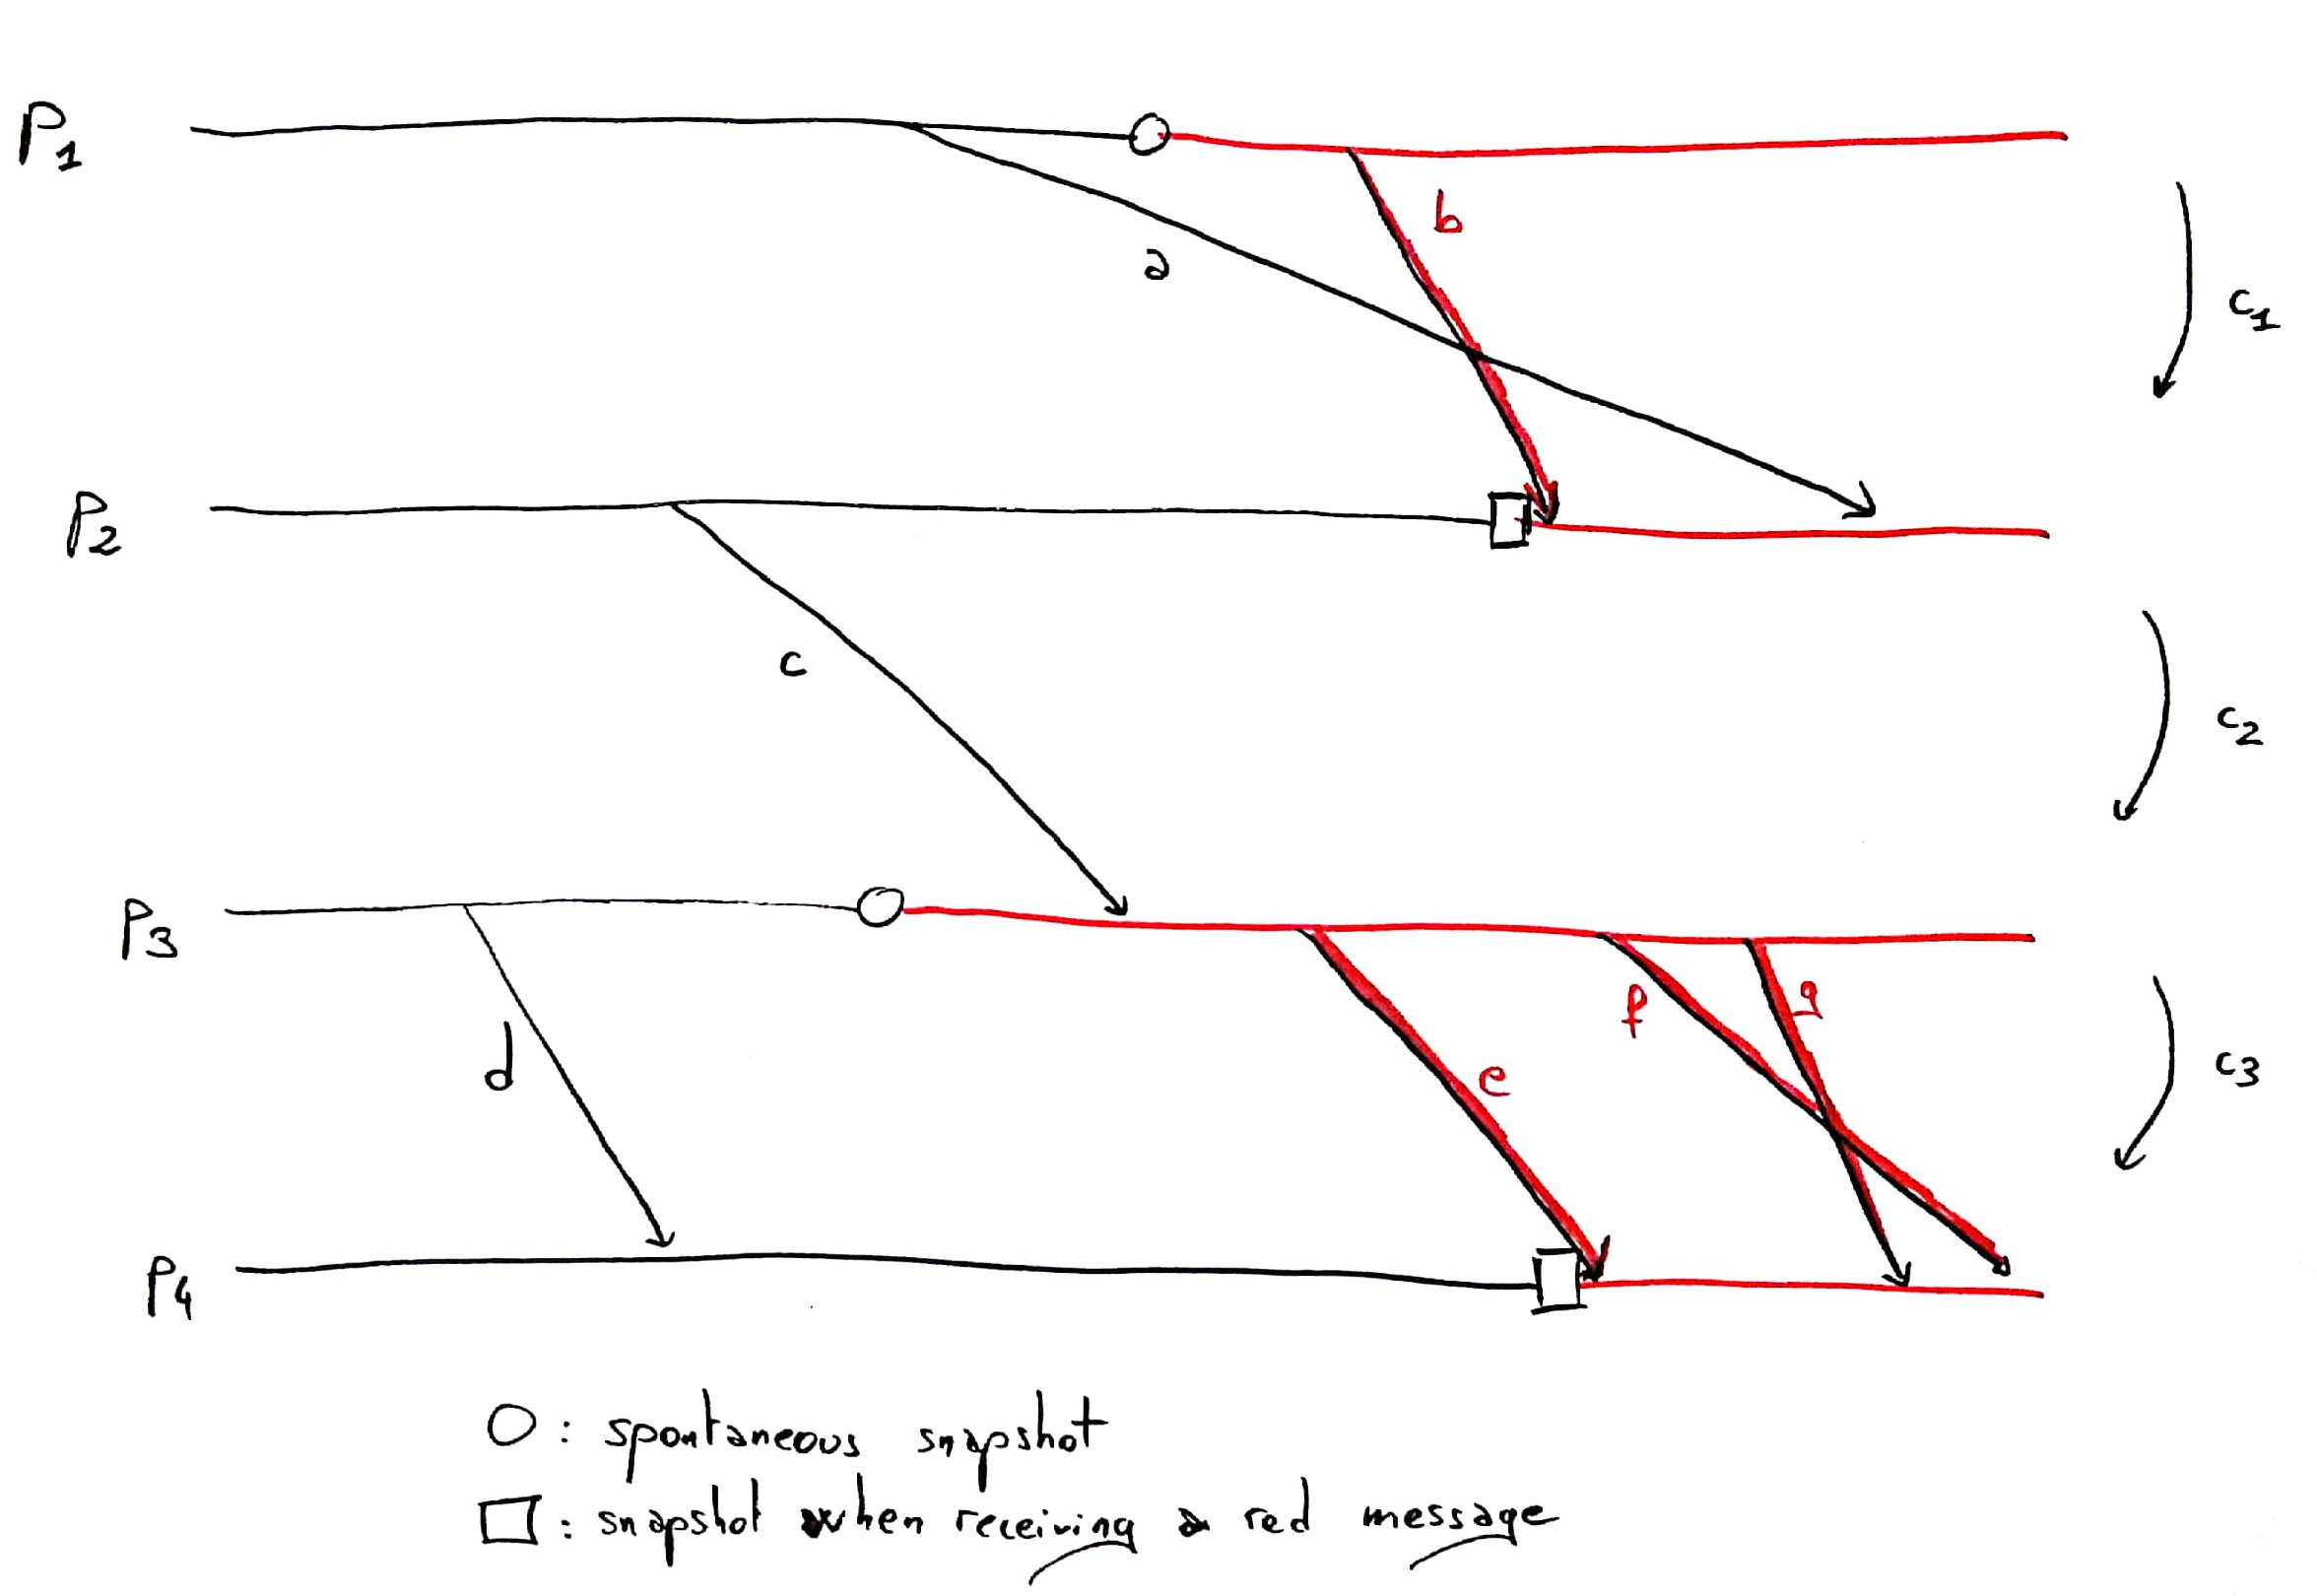
\includegraphics[scale=0.15]{example.jpg}
  \caption{An example execution of the algorithm}
\end{figure}

The system has 4 processes $p_1,p_2,p_3$ and $p_4$.
To simplify, we consider only the 3 channels $c_1=(p_1,p_2)$, $c_2=(p_2,p_3)$ and $(c_4=(p_3,p_4)$.
Of course, there needs to be more channels for the system to be strongly connected, but this will be enough for our example.
You can see with messages $a$ and $b$ that the channels aren't required to be FIFOs.
Messages $b,e,f$ and $g$ are colored red, while $a,c$ and $d$ are colored white.
Both processes $p_1$ and $p_3$ decide spontaneously to take a snapshot.
Process $p_2$ turns red and take a snapshot when receiving message $b$ (and before processing it).
Process $p_4$ does it when receiving message $e$ (and before processing it).

The global snapshot is the pair $(CC,PC)$ where
$PC(p_i)$ is the state of each $p_i$ at the time of its snapshot (not depicted here), and
\begin{itemize}
\item $CC(c_1)=\{a\}$
\item $CC(c_2)=\{c\}$
\item $CC(c_3)=\emptyset$
\end{itemize}

We get the following multisets at the time of each snapshot:
\begin{itemize}
\item $\mathit{sent}(p_1)=\{a\}$
\item $\mathit{received}(p_1)=\emptyset$
\item $\mathit{sent}(p_2)=\{c\}$
\item $\mathit{received}(p_2)=\emptyset$
\item $\mathit{sent}(p_3)=\{d\}$
\item $\mathit{received}(p_3)=\emptyset$
\item $\mathit{sent}(p_1)=\emptyset$
\item $\mathit{received}(p_1)=\{d\}$
\end{itemize}
Notice that each sent message has either been received, or is captured by the $CC$ function.


\section{Correctness proof}
\q{Prove correctness of the algorithm in your formal setting.}

For the algorithm to be correct, we want it to return a meaningful global snapshot.
According to \textbf{Theorem 3.1}, proved in the article, \textit{All feasible global snapshots are meaningful}.
Thus, it suffices to prove that the returned snapshot is feasible.

To do so, it is enough to prove the following:
$$\forall c=(p,q)\in C, \forall m\in M,\quad m\in\mathit{received}(q)\Rightarrow m\in\mathit{sent}(p)$$

Informally, it means that each received message in the snapshot has been sent in the snapshot. This corresponds to snapshots that are reachable global states of the distributed system.
Let $c=(p,q)\in C$, let $m\in\mathit{received}(q)$.
We first prove the following Lemma:\\
\textbf{Lemma 1:} $m$ is colored white.

As $m$ is in $\mathit{received}(q)$, it is enough to prove that, at the time of the snapshot, each message received was white. This holds because upon receiving a red message as a white process, the snapshot is taken before adding the message to the \lstinline{received} multiset.\\
\textbf{Lemma 2:} $m$ was sent when $p$ was white.

We can clearly see in the algorithm that messages are sent with the current color of the process. As $m$ is white, $p$ was white when the message was sent.\\
\textbf{Lemma 3:} Messages sent when a process is white $p$ are all included in $\mathit{sent}(p)$.

Indeed, the snapshot is always taken right before the process turns red.
It follows that $m\in\mathit{sent}(p)$.

Thus, the global snapshot returned by the algorithm is feasible, and meaningful.
In other words, each received message has been sent, and this has been captured in the snapshot as expected.

\section{Assumptions}
\q{What are the assumptions for the algo to work properly ? what if one releases these assumptions ?}

\textbf{Spontaneity.} The algorithm assumes that processes are able to spontaneously take a snapshot (with \lstinline{spontaneous_choice}). Without this assumption, no process may ever take a snapshot.

It is however enough to have only one spontaneous process. As the distributed system is a strongly connected graph, we could then have each process propagate the spontaneous choice until all have turned red.

\textbf{Prefect channels.} The algorithm assumes that no message can be lost or altered when going through a channel.
Without this assumption, the snapshot might not contain all messages, but is still meaningful.
However, when sending the local snapshots to the process in charge of building the global one, every message must reach its goal.

\textbf{Different Messages.} In the article, a set is maintained to represent the messages in each channel.
If two same messages are sent along the same channel, only one will be received. To avoid this issue, we used multisets of messages (that can have duplicates) in our formalism.

\section{Added complexity}
\q{What is the extra complexity due to the dropping the FIFO assumption, compared to Chandy-Lamport ?}

When taking a local snapshot, each process saves a copy of all sent and received messages.
For a single process to build the global snapshot, these two sets must be sent.
In Chandy-Lamport's algorithm, each process could locally compute the state of each incoming channel. The only control message required was a simple marker after each snapshot.

This could be an issue when taking series of snapshots. However, many properties only require sending the number of message sent, not the entire history.

Another extra complexity is the color of each message, but in most cases, adding one single bit by message should not be problematic.

\section{FIFO Channels}
\q{Does the algorithm simplify if channels are FIFO ?}

If channels are FIFO, the number of messages can be enough to identify the state of the channels.
For instance, if process $p$ has sent 12 messages along $c=(p,q)$ and p has received 8 at the time of the snapshot, then we know for sure that the 4 messages in the channel state are the 4 last ones.
If we assume that every process can communicate with the one in charge of building the global snapshot $p_{global}$, then for a channel $c=(p,q)$, $q$ could send the number of messages received to $p_{global}$, which in turn sends this number to $p$. $p$ can then compute the state of $c$ in the snapshot and sends it to $p_{global}$.
This way, we don't need to send all the previous history, but only some numbers and the part of the history that actually matters to build the global snapshot. This could be especially useful when taking series of snapshots.

\section{Deadlock or crash handling}
\q{Assuming a deadlock or a crash is detected, how should one resume computations from such a snapshot ?}

After a deadlock or a crash has been detected, it suffices to restore each process and each channel to a previous snapshot.
With a meaningful snapshot, each sent message has either been received, or is inside a channel, and each received message has been sent. This means that the distributed system can resume execution from there without losing or duplicating any message.
Each snapshot corresponds to a reachable global state.



\end{document}
